%%%%%%%%%%%%%%%%%%%%%%%%%%%%%%%%%%%%%%%%%%%%%%%%%%%%%%%%%%%%%%%%%%%%%
%
% Draft report Fuzzy Logic
%
%%%%%%%%%%%%%%%%%%%%%%%%%%%%%%%%%%%%%%%%%%%%%%%%%%%%%%%%%%%%%%%%%%%%%%

\documentclass[a4paper]{article}
\usepackage[utf8]{inputenc}
\usepackage[english]{babel}

\usepackage[myheadings]{fullpage}
\usepackage{fancyhdr}
\usepackage{lastpage}
\usepackage{graphicx, wrapfig, subcaption, setspace, booktabs}
\usepackage[font=small, labelfont=bf]{caption}
\usepackage{fourier}
\usepackage[protrusion=true, expansion=true]{microtype}

\usepackage{sectsty}

\newcommand{\HRule}[1]{\rule{\linewidth}{#1}}
\onehalfspacing
\setcounter{tocdepth}{5}
\setcounter{secnumdepth}{5}

\usepackage{amsmath}
\usepackage{hyperref}
\usepackage{lipsum}

%-------------------------------------------------------------------------------
% HEADER & FOOTER
%-------------------------------------------------------------------------------
\pagestyle{fancy}
\fancyhf{}
\setlength\headheight{15pt}
\fancyhead[L]{Peter Heemskerk, Stefan Schenk, Jim Kamans}
\fancyhead[R]{Draft Report}
\fancyfoot[R]{Page \thepage\ van \pageref{LastPage}}
%-------------------------------------------------------------------------------
% TITLE PAGE
%-------------------------------------------------------------------------------

\begin{document}

\title{ \normalsize \textsc{University of Amsterdam}
    \\ [2.0cm]
    \HRule{0.5pt} \\
    \LARGE \textbf{\uppercase{Draft Report Fuzzy Logic}}
    \HRule{2pt} \\ [0.5cm]
    \normalsize \today \vspace*{5\baselineskip}}

\date{}

\author{
    Authors: Peter Heemskerk, Stefan Schenk, Jim Kamans \\
    Studentnrs: \dots, 11881798, 10302905 \\
        Course: Fundamentals of Fuzzy Logic}

\maketitle
\newpage

\tableofcontents
\newpage

%-------------------------------------------------------------------------------
% Section title formatting
\sectionfont{\scshape}
%-------------------------------------------------------------------------------

%-------------------------------------------------------------------------------
% BODY
%-------------------------------------------------------------------------------
\section{Abstract}

Large organizations have problems with their customer service, since due to their complexity, they cannot answer messages from external parties in a quick manner. This project aims to demonstrate that Fuzzy Logic can be used to solve this problem, by determining the correct addressee within the organization in an automatic way.

In this project is has been demonstrated that Fuzzy Logic can successfully be implemented. The team implemented software based on a Python implementation.

\section{Introduction}

This work is done in autumn 2017 as part of the bachelor course Fundamentals of Fuzzy Logic by A. Bilgin (and  M. Hol and V. Dankers) within the study Artificial Intelligence at University of Amsterdam.

\subsection{Problem}
Many large organizations suffer from their own complexity. If an external party seeks contact with a specific person in an organization, this works fine, but if a party seeks contact about a subject (without knowing whom to talk to), it usually takes more time before the party gets a good answer. \\

Who has not have experience with this complexity or large organizations? Suppose you as a have a question on [example], we all have been facing either that we are sent from one person to another department (“kastje naar de muur”), or perhaps worse that we do not get answer at all, since the message is lost somewhere. Organization aim to get better on customer service, but tools who support this are building up. \\

This project aims to solve this issue of customer service in a complex organization. We present software based on fuzzy logic which aims to bring a message of an external party to the correct internal department or person fur further action, purely based on the content of the message. \\

Why fuzzy logic ?
\begin{itemize}
    \item First, with fuzzy logic methods, we can better deal with the uncertainties from the real world.
    \item Second, fuzzy logic deals well with incomplete or difficult to interpret data.
    \item Finally, fuzzy logic uses linguistic terms. With this we can include human knowledge into the system which is relatively easy to interpret.
\end{itemize}
These fuzzy and linguistic features support dealing with unstructured messages.

\subsection{Objectives}

Via several steps our software will bring a unstructured message (e-mail) to the correct department. For achieving this goal several steps are taken:
\begin{enumerate}
    \item from an email a list with relevant words is produced, irrelevant words are filtered out
    \item the words are matched and scored (word count) against a feature list
    \item with fuzzy logic these features are matched with a department.
    \item so the end result is a department attached to an email
\end{enumerate}

This project aims to prove that Fuzzy Logic works for this problem. Due to time-contraints the project has limitations:
\begin{itemize}
    \item Only written e-mails are used as input. At this moment e-mailing is the main way of communication to businesses (120billion/day) \ref{label-artikel}, and far more used that other ways like social media or message apps. This will change , so in later phase we envisage this to be expanded to messages in any other format, like messaging via Whatsapp or LinkedIn.
    \item The "word-to-feature translator" is implemented with limited scope, currently a number of only (xx?) English words. We did not extend to much on this, since we would like to focus on the Fuzzy Logic part of the software.
    \item We used a theoretical organization for the proposed structure of department, with first testing in the real world, we should test and amend this structure
\end{itemize}
\section{Literature reviews}

\textit{Provide a coherent and synthesized summary of relevant work in the
literature, present the supporting/related evidence for your project.} \\

\subsection{A Proactive Anti-Phishing Tool Using Fuzzy Logic and RIPPER Data Mining Classification Algorithm}

A Proactive Anti-Phishing Tool Using Fuzzy Logic and RIPPER Data Mining Classification Algorithm \cite{phishing} \\ is a paper that explains how phishing emails are detected using content- and non-content based approaches in the form of a combination of the RIPPER Classification Algorithm and a Fuzzy Logic system. The RIPPER Classifier is used to learn relations of the different phishing features, resulting into rules that are used by the Fuzzy Logic System. \\

While designing our system, the implementation of the content-based classification approach gives us a starting point for designing membership functions, linguistic variables and rules. However, the characteristics used to determine the crisp inputs aren't mentioned.

\subsection{A Content Based Classification of Spam Mails with Fuzzy Word Ranking}

A Content Based Classification of Spam Mails with Fuzzy Word Ranking
\cite{spam} introduces a different method by which a Fuzzy Logic System is used to categorize words that are spam in the degree to which these words are considered dangerous. The words are labeled to the names of five linguistic variables before they are fed to the particular input that corresponds with the name. After that, the Fuzzy Logic System outputs a degree of dangerousness. \\

This work seemed relevant before we finished our detailed design, but as our team gained more knowledge, it seemed that this approach misses all the value a Fuzzy Logic System is supposed to add.

\subsection{A new fuzzy logic based ranking function for efficient Information Retrieval system}

A new fuzzy logic based ranking function for efficient Information Retrieval system \cite{ranking} explains how "conventional ranking functions
fail to capture inherent features of documents and queries due to subjectivity
involved in natural language text", and offers a fuzzy approach to rank words
based on term-weighting schema's such as term frequency, inverse document
frequency and normalization. The tf/idf and normalization of the query and document are fed to their FLC (Fuzzy Logic Controller), whose outputs are fed to the main FLC, which in turn outputs a relevance score. \\

As we are using a content based approach in classifying emails, we need to determine whether words in the emails are related to words in a pre-assambled list.

\section{Approach}
In this section \dots

\subsection{Data}


\subsection{Design}

The solution consists of four main operations: Cleaning, Filterig, Ranking, and Classifying. These three terms are descriptive, but contain more additional steps that are somewhat corrolated to the meaning of the terms.

All actions in each step are represented by the colored arrows.

\begin{enumerate}
    \item Cleaning

    An email is read from the file system as plain text, containing mostly irrelevant information for classification. The text is tokenized, meaning that individual terms are stored as individual values. After that, capital characters are converted to lower case, punctuation and special characters are removed, resulting in an array of words.

    After that, stopwords are removed. Some examples of stopwords are: "a", "and", "but", "how", "or", and "what". And finally the words are stemmed, reducing words to their base root form. For example: "waited" will become "wait".

    \begin{figure}[ht!]
        \centering
        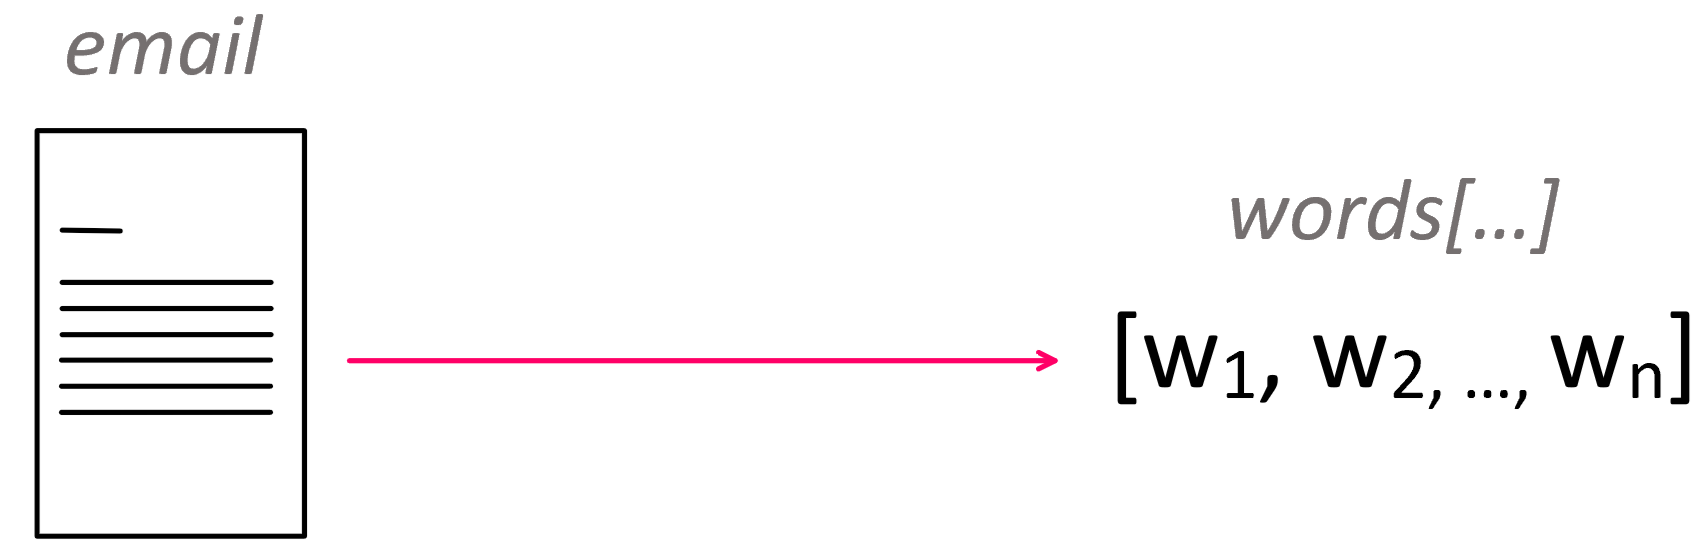
\includegraphics[width=.6\linewidth]{res/cleaning}
        \caption{Cleaning one email resulting into an array of words}
        \label{fig:sub1}
    \end{figure}

    \item Filtering

    The remaining words may be meaningfull now, but most of them may not be relevant. So the next operation will perform an intersection between the words and a list of predefined relevant words. All the words that reside in both lists will remain, but unlike sets, the list contains duplicates.

    As the last filtering step, the words are counted, and a corpus is created.

    \begin{figure}[ht!]
        \centering
        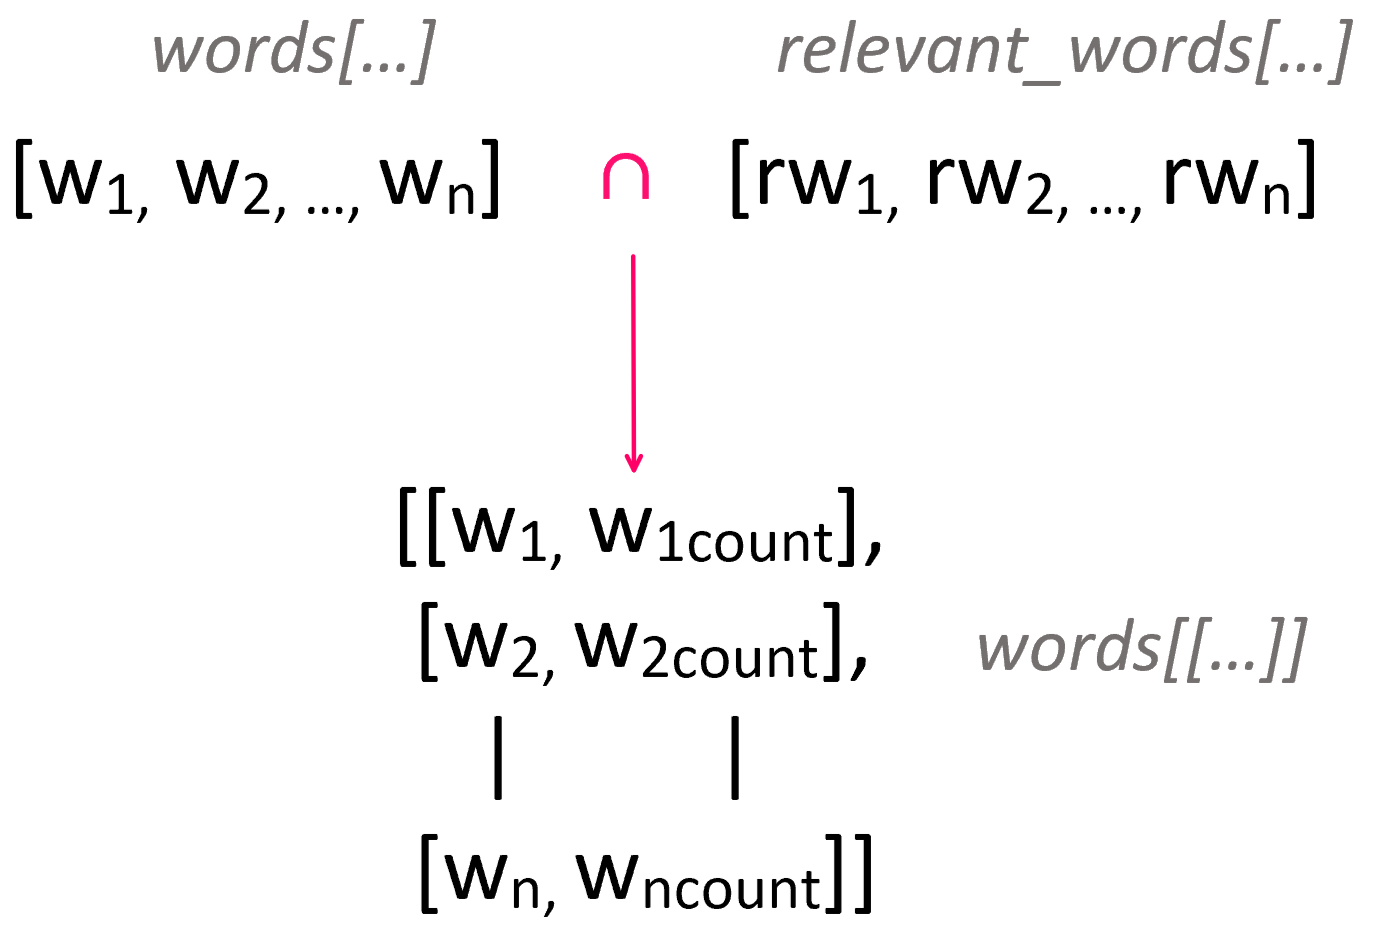
\includegraphics[width=.6\linewidth]{res/filtering}
        \caption{Taking the intersection of the words with a relevant list of words}
        \label{fig:sub1}
    \end{figure}

    \item Ranking

    Other predefined sets of words within the set of relevant words share the same characteristics. For example a set $T \subseteq R$ exists where $R$ is the set of technical words, and $R$ is the set of relevant words from before. Feature list of technical words: $T = [t_1, t_2, \dots, t_n]$.
    Other feature lists contain other themed words: $U$, $V$, $W$.

    For every word in the email that is present in $T$, a score is calculated that takes the count of that word into account in relation to the total number of relevant words in the email. This calculation is made for all feature lists ($T$, $U$, $V$, $W$), for every word in the email.

    \begin{figure}[ht!]
        \centering
        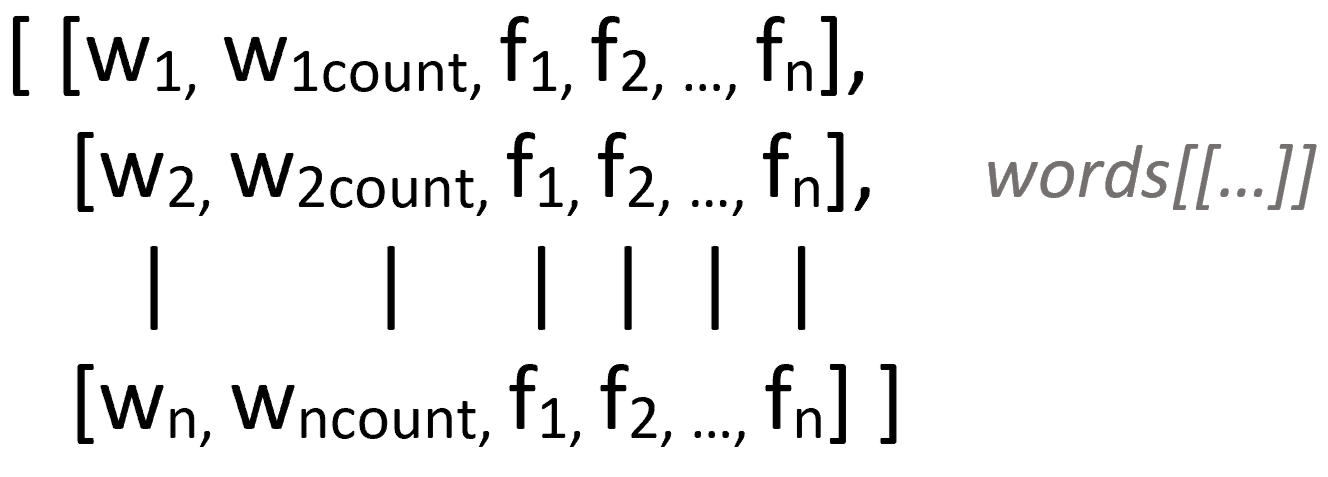
\includegraphics[width=.6\linewidth]{res/ranking}
        \caption{The scores for each words are added as features}
        \label{fig:sub1}
    \end{figure}

    \item Classifying

    Finally the scores are aggregated, resulting in the inputs for the Fuzzy Logic System.

\end{enumerate}


\subsection{Implementation}

%-------------------------------------------------------------------------------
% BIBLIOGRAPHY
%
% EX:
% \cite{citation1}
%
% \bibitem{citation1}
%     Leslie Lamport,
%     \textit{\LaTeX: a document preparation system},
%     Addison Wesley, Massachusetts,
%     2nd edition,
%     1994.
%-------------------------------------------------------------------------------
\begin{thebibliography}{9}

\bibitem{spam}
    G. Santhi, S. Maria Wenish, Dr. P. Sengutuvan,
    \textit{
        \href{https://github.com/Menziess/Fuzzy-Logic-Email-Classification/raw/master/report/res/a_content_based_classification_of_spam_mails_with_fuzzy_word_ranking.pdf}{A Content Based Classification of Spam Mails with Fuzzy Word Ranking},
    }
    Department of Information Science and Technology,
    Issue 3,
    2013.

\bibitem{phishing}
    Rosana J. Ferolin,
    \textit{
        \href{https://github.com/Menziess/Fuzzy-Logic-Email-Classification/raw/master/report/res/a_proactive_anti-phishing_tool_using_fuzzy_logic_and_ripper_data_mining_classification_algorithm.pdf}{A Proactive Anti-Phishing Tool Using Fuzzy Logic and RIPPER Data Mining Classification Algorithm},
    }
    Department of Computer Engineering University of San Carlos.

\bibitem{ranking}
    Rosana J. Ferolin,
    \textit{
        \href{https://github.com/Menziess/Fuzzy-Logic-Email-Classification/raw/master/report/res/a_new_fuzzy_logic_based_ranking_function_for_efficient_information_retrieval_system.pdf}{A new fuzzy logic based ranking function for efficient Information Retrieval system},
    }
    Department of Electrical Engineering Dayalbagh Educational Institute,
    2014.

\end{thebibliography}

\end{document}
